\section{\bf The geometry of calculus of variations}
\subsection{The geometric setting}
\begin{frame}
    \frametitle{The geometric setting I}
    \begin{center}
        {\large \bf What to minimize/maximize? \alert{Sections!}}
    \end{center}
    Fixed some fibered manifold $$Y \xrightarrow{\pi_{YX}} X \,\, \text{with coordinates } (x^\mu, y^i) \mapsto x^\mu,$$
    we want to find a section $$\phi: X \rightarrow Y,\,\,  (x^\mu) \mapsto (x^\mu, y^i = \phi^i(x^\mu))$$
    minimizing/maximizing the functional $$\mathcal{J}[\phi] = \int_X L\left (x^\mu, \phi^i(x^\mu), \pdv{\phi^i}{x^\mu}, \pdv{\phi^i}{x^\mu}{x^\nu},\dots\right ) d^n x.$$
    We will focus on \alert{first order} theories,
    $$\mathcal{J}[\phi] = \int_X L\left (x^\mu, \phi^i(x^\mu), \pdv{\phi^i}{x^\mu} \right ) d^n x.$$ 
\end{frame}

\begin{frame}
    \frametitle{The geometric setting II}
    We can interpret  $$L\left (x^\mu, \phi^i(x^\mu), \pdv{\phi^i}{x^\mu} \right ) d^n x$$
    as an $n$-form on the first jet bundle $$J^1 \pi_{YX} \text{ with coordinates } (x^\mu, y^i, z^i_\mu).$$ We 
    call it \alert{the Lagrangian density} $$\mathcal{L} = L(z^\mu, y^i, z^i_\mu) d^nx.$$ We can rewrite the action as 
    $$\mathcal{J}[\phi] = \int_X (j^1 \phi)^\ast \mathcal{L}.$$
\end{frame}

\begin{frame}
    \centering
    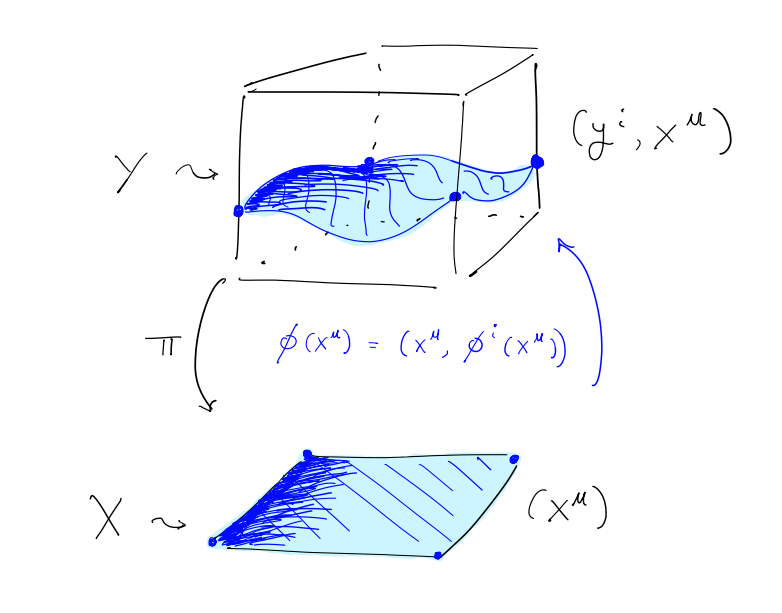
\includegraphics[width = 250pt]{Images/Variational_problem.PNG}
    $$\mathcal{J}[\phi] = \int_X (j^1\phi)^\ast \mathcal{L},$$
    where $\mathcal{L} \in \Omega^n(J^1  \pi_{YX})$ is the Lagrangian dentisy.
\end{frame}

\subsection{The Euler-Lagrange equations}
\begin{frame}
    \frametitle{The Euler-Lagrange equations I}
    If $\phi$ is a minimizer/maximizer (more generally, \alert{stationary section}), 
    $$\dv{t}\bigg |_{t = 0} \mathcal{J}[\textcolor{red}{\phi_t}] = 0, \, \forall \text{ variation } \textcolor{red}{\phi_t}.$$
    \begin{center}
        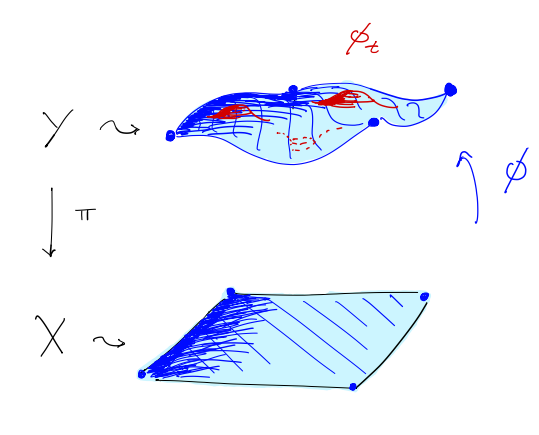
\includegraphics[width = 210pt]{Images/Variations.PNG}
    \end{center}
\end{frame}

\begin{frame}
    \frametitle{The Euler-Lagrange equations II}
    Equivalently, $$0 = \int_X \dv{t}\bigg |_{t = 0} (j^1\textcolor{red}{ \phi_t})^\ast \mathcal{L}.$$
    Locally, we get $$\pdv{L}{y^i} = \dv{x^\mu} \left ( \pdv{L}{z^i_\mu} \right ).$$ 
    \begin{center}
        {\large \bf What about \alert{intrinsic} Euler-Lagrange equations?}
    \end{center}
    If we define
    $$\textcolor{red}{\xi} := \dv{t}\bigg |_{t = 0} \textcolor{red}{\phi_t} = \xi^i \pdv{y^i} \in \mathfrak{X}(Y),$$
    $$\textcolor{red}{\xi^{(1)}} := \dv{t}\bigg |_{t = 0} j^1\textcolor{red}{\phi_t} = \xi^i \pdv{y^i} + \left(\pdv{\xi^i}{x^\mu} + \pdv{x^i}{y^j} z^j_\mu \right) \pdv{z^j_\mu}\in \mathfrak{X}(J^1 \pi_{YX}).$$
\end{frame}

\begin{frame}
    \frametitle{The Euler-Lagrange equations III}
    If we define
    $$\textcolor{red}{\xi} := \dv{t}\bigg |_{t = 0} \textcolor{red}{\phi_t} = \xi^i \pdv{y^i} \in \mathfrak{X}(Y),$$
    $$\textcolor{red}{\xi^{(1)}} := \dv{t}\bigg |_{t = 0} j^1\textcolor{red}{\phi_t} = \xi^i \pdv{y^i} + \left(\pdv{\xi^i}{x^\mu} + \pdv{x^i}{y^j}
     z^j_\mu \right) \pdv{z^j_\mu}\in \mathfrak{X}(J^1 \pi_{YX}),$$
    
    $$0 = \dv{t}\bigg |_{t = 0} \mathcal{J}[\textcolor{red}{\phi_t}] = \int_X (j^1 \phi)^\ast \pounds_{ \textcolor{red}{\xi^{(1)}}}
     \mathcal{L}, \, \text{for every vertical } \textcolor{red}{\xi} \in \mathfrak{X}(Y)$$
    Applying Stokes' Theorem
    $$0 = \int_X (j^1 \phi)^\ast  \iota_{ \textcolor{red}{\xi^{(1)}}}
     d \mathcal{L} + \int_X d \iota_{ \textcolor{red}{\xi^{(1)}}}
     \mathcal{L} = \int_X (j^1 \phi)^\ast  \iota_{ \textcolor{red}{\xi^{(1)}}}
     d \mathcal{L}.$$
\end{frame}

\begin{frame}
    \frametitle{The Euler-Lagrange equations IV}
    $$0 = \int_X (j^1 \phi)^\ast  \iota_{ \textcolor{red}{\xi^{(1)}}}
     d \mathcal{L}\,\, \text{for every vertical } \textcolor{red}{\xi} \in \mathfrak{X}(Y).$$
    \alert{Does not yield equations.}
    \begin{center}
        {\large \bf \alert{Idea}: modify $\mathcal{L}$}
    \end{center}
    We want to find an $n$-form $\Theta_\mathcal{L}$ satisfying $$(j^1 \phi)^\ast \mathcal{L} = (j^1 \phi)^\ast \Theta_\mathcal{L}$$
    such that $\phi$ is an stationary field of the action if and only if
    $$0 = \int_X (j^1 \phi)^\ast  \iota_{ \textcolor{blue}{\eta}}
     d \Theta_\mathcal{L}\,\, \text{for every } \textcolor{blue}{\eta} \in \mathfrak{X}(J^1 \pi_{YX}).$$
\end{frame}

\begin{frame}
    \frametitle{The Euler-Lagrange equations V}
    \begin{proposition} There is such $\Theta_\mathcal{L}$, and can be intrinsically defined (using the geometry of $J^1 \pi_{YX}$).
    \end{proposition}
    Locally, 
    $$\Theta_\mathcal{L} =  \pdv{L}{z^i_\mu}  dy^i \wedge d^{n-1}x_\mu - \left( \pdv{L}{z^i_\mu}z^i_\mu - L \right) d^n x$$
    and it is called \alert{the Poincaré-Cartan form}.

    \begin{corollary}[Intrinsic Euler-Lagrange equations]
        A field $\phi:X \rightarrow Y$ is stationary if and only if it satifies
        $$(j^1 \phi)^\ast \iota_{\textcolor{blue}{\eta}} d\Theta_\mathcal{L} = 0, \,\,\text{for every } \textcolor{blue}{\eta} \in \mathfrak{X}(J^1 \pi_{YX}).$$
    \end{corollary}
\end{frame}

\begin{frame}
    \frametitle{Looking for solutions}
    To find solutions, we can look for distributions on $J^1 \pi_{YX} \rightarrow$ such that an integral
    section of such this distribution $\sigma: X \rightarrow J^1 \pi_{YX}$ satisfies $$\sigma^\ast \iota_\eta \Omega_\mathcal{L} = 0, \forall \eta \in \mathfrak{X} (J^1 \pi_{YX}).$$
    We can define such distributions via decomposable $n$-multivector fields $$U = X_1 \wedge \cdots \wedge X_n.$$
    \begin{center}
        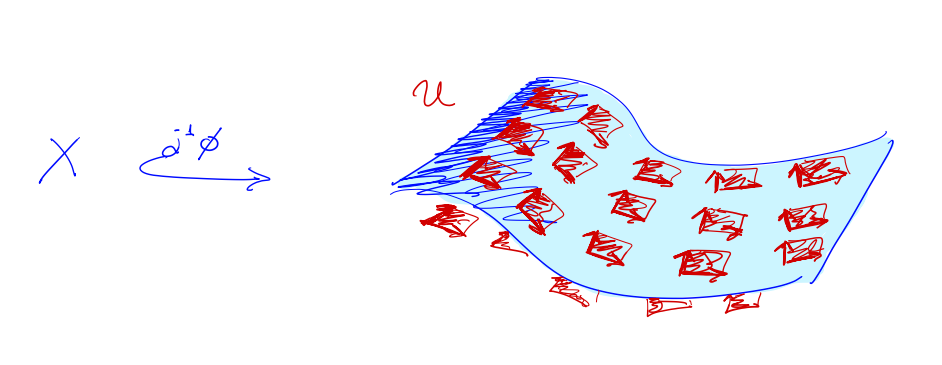
\includegraphics[height = 100pt]{Images/Multivector_multisymplectic.PNG}
    \end{center} 
    Then, being stationary is characterized by $\iota_U \Omega_\mathcal{L} = 0$.
\end{frame}

\begin{frame}
    \frametitle{Disclaimer}
    Giving such a multivector field $U$ does not immediately give a solution:
    \begin{itemize}
        \item We need to make sure that the corresponding distribution is integrable.
        \item Even if it is integrable, it may not be holonomic. That is, that the corresponding 
        integral section $\sigma: X \rightarrow J^1 \pi_{YX}$ could fail to be the jet lift of some section $$\phi: X \rightarrow Y.$$
        When $\mathcal{L}$ is \alert{regular,} this is not an issue.
        \item Even if it satisfies the previous conditions, there may not exist global sections of $Y \xrightarrow{\pi_{YX}} X$.
    \end{itemize}
\end{frame}

\begin{frame}
    \frametitle{Summary}
    \begin{itemize}
        \item Fields, denoted by $\phi$, are sections of a fibered manifold $Y \xrightarrow{\pi_{YX}} X.$
        \item A first order variational problem is defined through a Lagrangian density $\mathcal{L}$ 
         on $J^1 \pi_{YX}$ (which defines an $n$-form on $X$ at each point), and the action can be expressed as
        $$\mathcal{J}[\phi] = \int_X (j^1 \phi)^\ast \mathcal{L}.$$
        \item If we define the \alert{multisymplectic form} as $$\Omega_\mathcal{L} := -d \Theta_\mathcal{L},$$
        stationary fields are characterized by $$(j^1 \phi)^\ast \iota_{\eta} \Omega_\mathcal{L} = 0, \,\, \text{for every } \eta \in \mathfrak{X}(J^1 \pi_{YX}).$$
        In particular, we can look for decomposable horizontal $n$-multivector fields $U$ satisfying $$\iota_U \Omega_\mathcal{L} = 0.$$
    \end{itemize}
\end{frame}
